% META: DONE.1

\section{Измерение быстродействия итоговой системы}

\subsection{Оборудование}

Аппаратное обеспечение:

\begin{itemize}
    \item CPU: 13th Gen Intel(R) Core(TM) i9-13900HX (24 ядра: 8 P-cores до 5.4 ГГц, 16 E-cores до 3.9 ГГц)
    \item RAM: 64 GB DDR5-4800 (двухканальный режим)
    \item GPU: NVIDIA GeForce RTX 4090 Laptop GPU (16 GB GDDR6, 9728 CUDA ядер, 304 Tensor ядра)
    \item Накопитель: NVMe SSD (произвольные замеры I/O не критичны)
\end{itemize}

Программное окружение (Linux/Python):

\begin{itemize}
    \item ОС: Ubuntu 24.04.4 LTS
    \item Python: 3.12.2
    \item PyTorch: 2.6.0+cu124
    \item CUDA: 12.4
    \item cuDNN: 9.0.1 (90100)
    \item NVIDIA драйвер: 580.126.09
\end{itemize}



\subsection{Обучение}

В таблице \ref{tab:time-train} представлено время, затраченное на обучение нейронных сетей различных конфигураций на разных датасетах. Видно, что задача классификации (конфигурации a и b) занимает почти в 2 раза меньше времени на обучение, чем задача сегментации (конфигурации c, d и e). При этом нет прямой зависимости между числом параметров и временем обработки одной модели - вероятно, это связано с тем, что разные параметры влияют на количество параметров совершенно по-разному. Требуются дополнительные исследования для более точного определения времени работы.

\begin{table}[h]
\centering
\small
\begin{tabular}{|p{0.2\linewidth}|p{0.15\linewidth}|p{0.15\linewidth}|p{0.1\linewidth}|p{0.1\linewidth}|p{0.15\linewidth}|}
\hline
Конфигурация & Операция & Число моделей & Число эпох & Время (мин.) & Среднее время на модель на эпоху (мс) \\
\hline
\multirow{3}{*}{a} & cutExtrusion  & 3323 & 20 & 49.89  & 45.04  \\
                   & fillet        & 1996 & 20 & 29.75  & 44.71 \\
                   & chamfer       & 2971 & 20 & 45.3   & 45.74 \\
\hline
\multirow{3}{*}{b} & cutExtrusion  & 3323 & 20 & 58.31  & 52.64 \\
                   & fillet        & 1996 & 20 & 34.55  & 51.93 \\
                   & chamfer       & 2971 & 20 & 51.78  & 52.29 \\
\hline
\multirow{3}{*}{c} & cutExtrusion  & 3031 & 50 & 220.92 & 87.46 \\
                   & fillet        & 919  & 50 & 62.34  & 81.4 \\
                   & chamfer       & 1376 & 50 & 92.46  & 80.63 \\
                   & bossExtrusion & 1330 & 50 & 92.52  & 83.48 \\
\hline
\multirow{3}{*}{d} & cutExtrusion  & 3031 & 50 & 275.4  & 109.03 \\
                   & fillet        & 919  & 50 & 85.2   & 111.25 \\
                   & chamfer       & 1376 & 50 & 115.5  & 100.73 \\
                   & bossExtrusion & 1330 & 50 & 110.28 & 99.5 \\
\hline
\multirow{3}{*}{e} & cutExtrusion  & 3031 & 50 & 195.84 & 77.53 \\
                   & fillet        & 919  & 50 & 59.7   & 77.95 \\
                   & chamfer       & 1376 & 50 & 88.08  & 76.81 \\
                   & bossExtrusion & 1330 & 50 & 87.18  & 78.66 \\
\hline
\end{tabular}
\caption{Замер времени обучения нейронных сетей}
\label{tab:time-train}
\end{table}



\subsection{Инференс}

\subsubsection{Linux, python}

В таблице \ref{tab:time-inference-linux} представлено время, затраченное на инференс различных конфигураций на тестовой модели. Тестовая модель представляет собой куб, с несколькими фасками и круглым сквозным отверстием посередине (рисунок \ref{fig:test_model}). Исходя из таблицы, примерно 500 мс требуется программе на предобработку STP файла, после чего примерно 2200 мс требуется на полную инициализацию и обработку нейронными сетями. Также, отсутствуют значимые различия между запусками различных конфигураций, что, скорее всего, связано с маленьким размером запускаемых нейронных сетей.

\begin{table}[h]
\centering
\small
\begin{tabular}{|p{0.25\linewidth}|p{0.15\linewidth}|p{0.15\linewidth}|}
\hline
Конфигурация & {Кэш} & {Без кэша} \\
\hline
a & 2318.694 & 2759.324 \\
b & 2223.696 & 2817.746 \\
c & 2310.911 & 2859.118 \\
d & 2226.515 & 2779.992 \\
e & 2163.540 & 2769.299 \\
\hline
\end{tabular}
\caption{Замер времени инференса (Linux, python)}
\label{tab:time-inference-linux}
\end{table}

\begin{figure}[h]
    \centering
    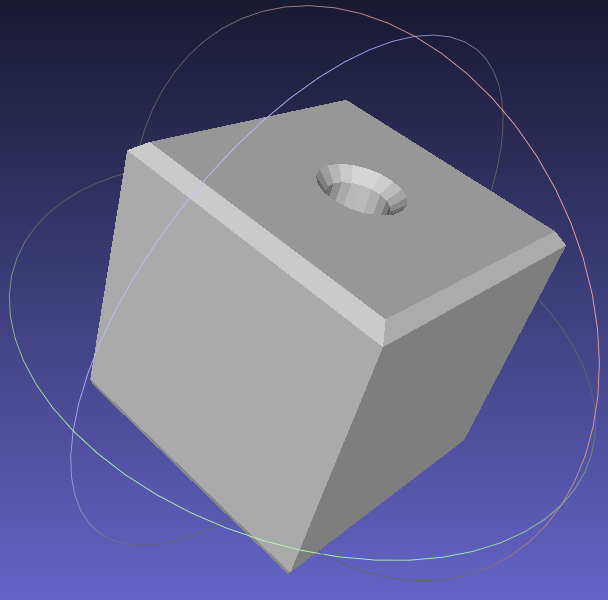
\includegraphics[width=0.8\linewidth]{figures/test_model.png}
    \caption{Тестовая модель для проверки времени работы инференса}
    \label{fig:test_model}
\end{figure}

\subsubsection{Windows, exe}

В таблице \ref{tab:time-inference-windows} представлено время, затраченное на инференс различных конфигураций на тестовой модели. Исходя из таблицы, примерно 550 мс требуется программе на предобработку STP файла, после чего примерно 3400 мс требуется на полную инициализацию и обработку нейронными сетями. Также, отсутствуют значимые различия между запусками различных конфигураций, за исключением конфигурации c - что, скорее всего, является выбросом.

\begin{table}[h]
\centering
\small
\begin{tabular}{|p{0.25\linewidth}|p{0.15\linewidth}|p{0.15\linewidth}|}
\hline
Конфигурация & {Кэш} & {Без кэша} \\
\hline
a & 3382.11645 & 3912.18895 \\
b & 3413.94006 & 3900.16413 \\
c & 3757.00126 & 4436.62332 \\
d & 3493.56021 & 4080.72251 \\
e & 3339.23962 & 4015.50719 \\
\hline
\end{tabular}
\caption{Замер времени инференса (Windows, exe)}
\label{tab:time-inference-windows}
\end{table}

\subsubsection{Итоги}

Таким образом, исходя из того, что время, затраченное на предобработку файлов, примерно одинаково, можно предположить, что разница в 3400 - 2200 = 1200 мс объясняется задержкой перед выполнением, связанным с инициализацией python изнутри exe файла. Итоговые затраты по времени включают:

\begin{itemize}
    \item 1200 мс требуется на инициализацию на Windows;
    \item 500 мс требуется на инициализацию;
    \item 1700 мс требуется на полную обработку нейронными сетями.
\end{itemize}

Постобработка занимает незначительное время, поэтому получить достоверных данных по времени выполнения не удалось.

